\section{eo\-Bit\-Inversion$<$ Chrom $>$ Class Template Reference}
\label{classeo_bit_inversion}\index{eoBitInversion@{eoBitInversion}}
eo\-Bit\-Inversion: inverts the bits of the chromosome between an interval  


{\tt \#include $<$ga/eo\-Bit\-Op.h$>$}

Inheritance diagram for eo\-Bit\-Inversion$<$ Chrom $>$::\begin{figure}[H]
\begin{center}
\leavevmode
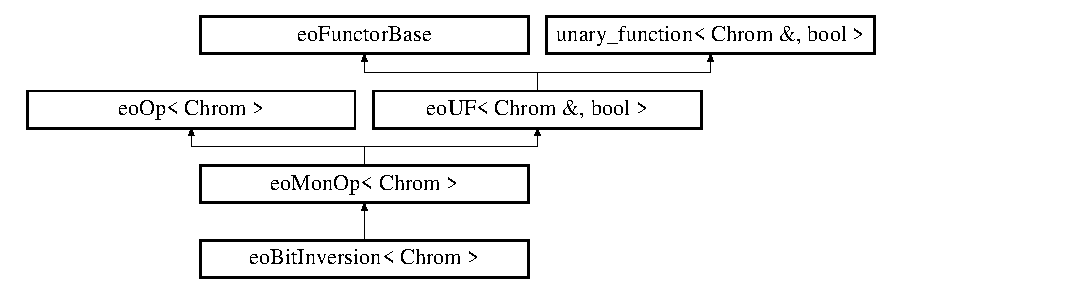
\includegraphics[height=3.50548cm]{classeo_bit_inversion}
\end{center}
\end{figure}
\subsection*{Public Member Functions}
\begin{CompactItemize}
\item 
virtual std::string {\bf class\-Name} () const \label{classeo_bit_inversion_a0}

\begin{CompactList}\small\item\em The class name. \item\end{CompactList}\item 
bool {\bf operator()} (Chrom \&chrom)
\begin{CompactList}\small\item\em Inverts a range of bits in a binary chromosome. \item\end{CompactList}\end{CompactItemize}


\subsection{Detailed Description}
\subsubsection*{template$<$class Chrom$>$ class eo\-Bit\-Inversion$<$ Chrom $>$}

eo\-Bit\-Inversion: inverts the bits of the chromosome between an interval 



Definition at line 146 of file eo\-Bit\-Op.h.

\subsection{Member Function Documentation}
\index{eoBitInversion@{eo\-Bit\-Inversion}!operator()@{operator()}}
\index{operator()@{operator()}!eoBitInversion@{eo\-Bit\-Inversion}}
\subsubsection{\setlength{\rightskip}{0pt plus 5cm}template$<$class Chrom$>$ bool {\bf eo\-Bit\-Inversion}$<$ Chrom $>$::operator() (Chrom \& {\em chrom})\hspace{0.3cm}{\tt  [inline, virtual]}}\label{classeo_bit_inversion_a1}


Inverts a range of bits in a binary chromosome. 

\begin{Desc}
\item[Parameters:]
\begin{description}
\item[{\em chrom}]The chromosome whos bits are going to be inverted (a range). \end{description}
\end{Desc}


Implements {\bf eo\-UF$<$ Chrom \&, bool $>$} {\rm (p.\,\pageref{classeo_u_f_a1})}.

Definition at line 156 of file eo\-Bit\-Op.h.

The documentation for this class was generated from the following file:\begin{CompactItemize}
\item 
eo\-Bit\-Op.h\end{CompactItemize}
